\section{ Athena System}
%\section{System Framework}
\label{sec-system}

In this section, we introduce our \oursystem system.
As shown in Figure \ref{fig:framework}, \oursystem consists of three main components, \ie \emph{storage}, \emph{query engine} and {\em function modules}.
Below the storage component is a {\em query independent ranking} module that enriches the scholarly data with pre-computed query independent ranking scores,  there is another {\em query dependent ranking} module inside the query engine, and the two function modules support visual analyses for users.


%In this section, we introduce our \oursystem system. The system contains framework and schema, as shown in Figure \ref{fig:system}. The framework of \oursystem consists of three main components, \ie \emph{storage}, \emph{query engine} and {\em function modules} (Figure \ref{fig:framework}). The \emph{schema} is designed to model scholarly data as a property graph (Figure \ref{fig:schema}).

We next explain our system in detail.





\subsection{Schema Design} \label{subsec:schema}

Graph database Neo4j is adopted for storage in \oursystem. To do so, we need to design a schema that abstracts the entities and linked structures (\eg citation, authored-by).
% schema design rationaile
We follow two principles for schema design: (1) nodes for entities and relationships for linked structures, and (2) trading space for query efficiency if affordable and possible.

%reducing fine-grained relationship names while increase generic relationships qualified with property appropriately.

The schema is presented in Figure~\ref{fig:schema}, where the texts near nodes and relationships represent the properties of entities and linked structures, respectively.
It contains seven basic types of nodes including {\em Article}, {\em Author}, {\em Affiliation}, {\em Venue}, {\em FOS} (field of study), {\em ConIns} (conference instance in each year) and {\em Year}.
In addition, it further incorporates an artificial type of nodes, \ie~{\em AAA} representing article-author-affiliation tuples. Here we trade extra space for query efficiency, \ie an author and her/his affiliations can be retrieved in one query.
As another space-efficiency trade-off, we also use extra space to maintain certain properties of  {\em article} nodes: conference ID, journal ID and year.
%
Our schema also forms a total of nine types of relationships, one of which, \ie~{\em :VenueScore}, has a {\em score} property.



\begin{figure}
\centering
\subfigure[{\scriptsize \marked{Framework} }]{\label{fig:framework}
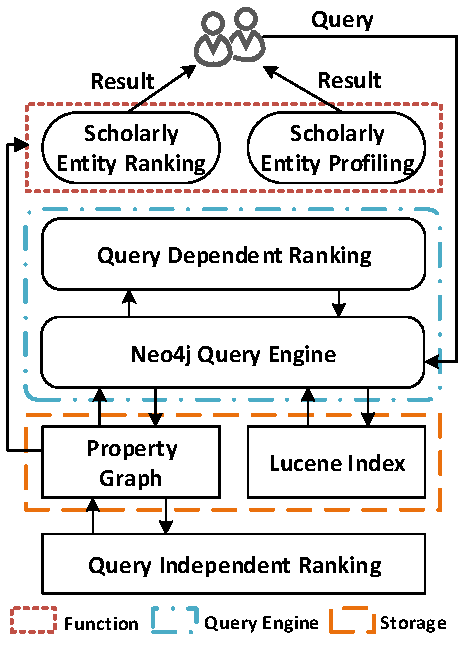
\includegraphics[width=0.45\columnwidth]{systemFrame.pdf}}
%\hspace{3ex}
\subfigure[{\scriptsize Neo4j schema}]{\label{fig:schema}
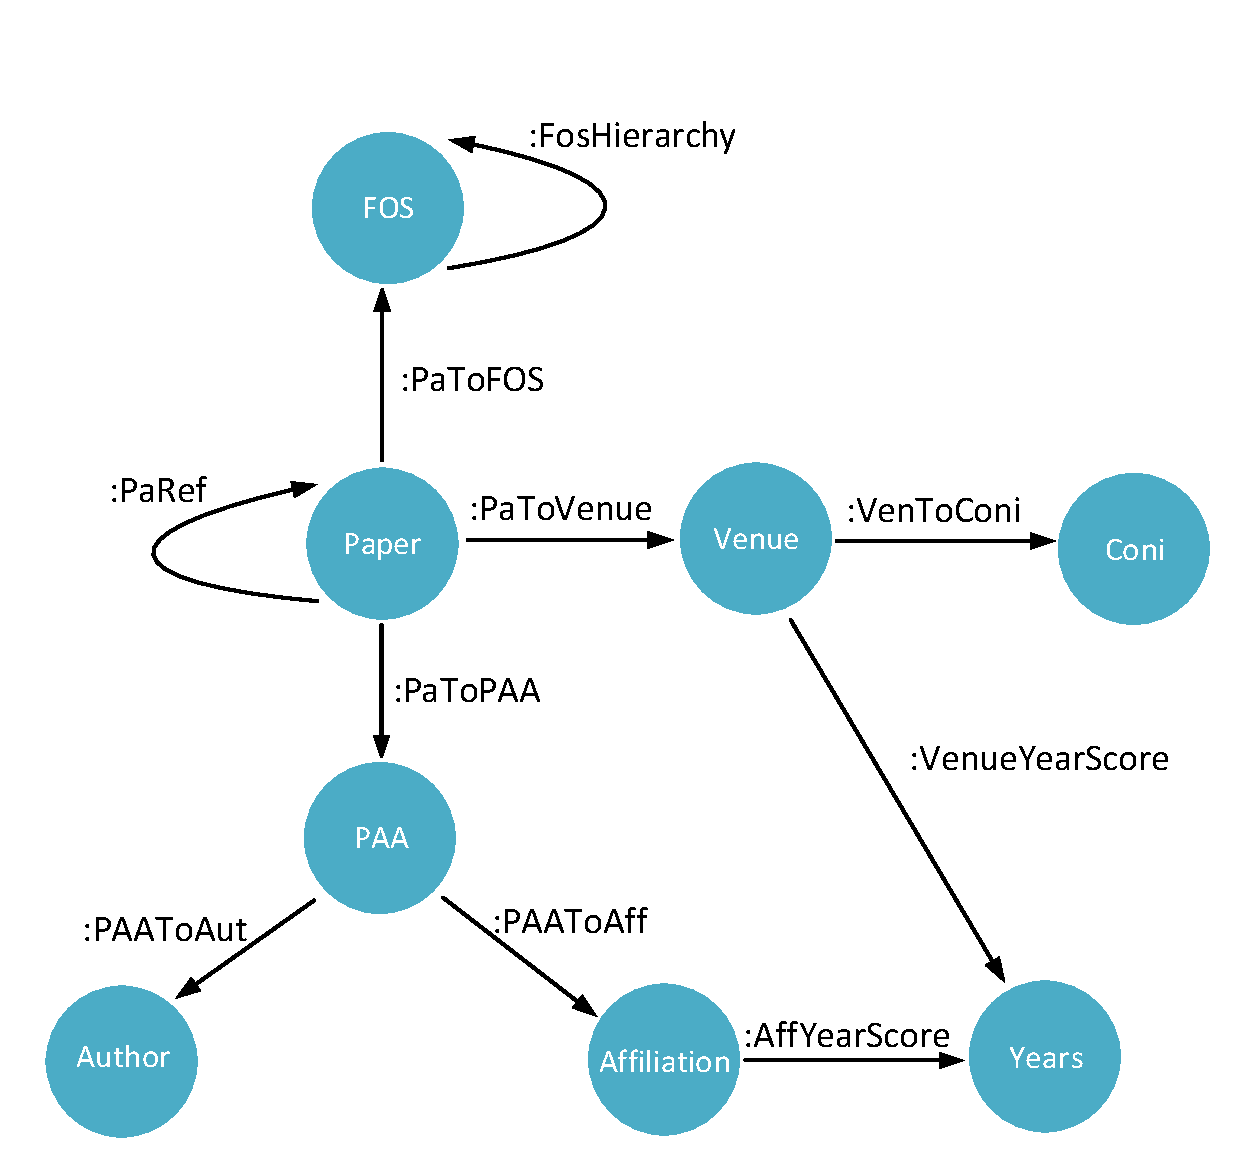
\includegraphics[width=0.5\columnwidth]{neo4jSchema.pdf}}
\vspace{-2ex}
\caption{System design of \oursystem  }
\label{fig:system}
\vspace{-2ex}
\end{figure}


\subsection{Graph Storage} \label{subsec:storage}


Following the above schema, we maintain scholarly data as a huge property graph, \eg the one of MAG~\cite{sinha2015overview}  has more than 1.03 billion nodes and 1.93 billion relationships. %We further clarify our graph storage with the following.


First, based on the original scholarly data, the {\em query independent ranking} module pre-computes those query independent ranking scores: citation counts of articles, importance scores of articles, authors, venues and affiliations~\cite{ma2018query}. These scores are assigned as properties to the corresponding nodes.
%As iteratively accessing the linked entities is the most essential operation in the pre-computation, the graph storage is much more convenient and effective for such computations.
\marked{
Moreover, both citation counts and importance scores support incremental computation~\cite{ma2018query}, and they are easy to be dynamically maintained once new scholarly data arrives.%once the property graph gets updated.
}


Second, to facilitate query processing on the billion-scale property graph, Lucene index is utilized for initial entity lookups. Specifically, we create fulltext indices for article titles, author names, venue names and affiliation names. These enable to efficiently find articles, authors, venues and affiliations whose titles or names contain specific keywords. %Besides, we also create schema indices for the entire author and venue names to speed up initial entity lookups.


\subsection{Graph Query Engine } \label{subsec:qe}
%Utilizing Neo4j, \oursystem supports a variety of graph queries on the property graph to aid scholarly search. And the {\em query engine} is responsible for processing this set of queries. When a query is issued, the {\em Neo4j query engine} first translates it into a Neo4j Cypher query with proper parsing and semantic analyses. When applicable, the Cypher query also includes the entity IDs returned from the Lucene index. Relevance and relevant importance rankings given by the {\em query dependent ranking} module may also be included in the Cypher query if needed.Based on the final Cypher query, an optimized query plan is generated and processed on the property graph.

% why graph queries: query involved with multiple types of entities --> join

\marked{
Complex scholarly queries, such as finding the top-$k$ fields of study of an author, inevitably involve with multiple types of entities. In RDBMS these are implemented with joins, which may become a bottleneck for query processing.
Differently, \oursystem executes graph queries on the property graph to answer scholarly queries.
}
\marked{
To be specific, when user issue a query, \oursystem first translates it into a Neo4j Cypher query.}

When applicable, the Cypher query also includes the entity IDs returned from the Lucene index. Relevance and relevant importance rankings given by the {\em query dependent ranking} module may also be included in the Cypher query if needed.
\marked{
Based on the final Cypher query, Neo4j query engine generates a query plan and processes it on the property graph after proper parsing and semantic analyses.
}

% Reviewer 2
% However, they do not specify what kind of graph queries are required and why it is challenging to evaluate them efficiently.
% specify graph queries. clear User Query and Neo4j Cypher Query.


%Figure~\ref{fig:queryProcess}
%Table~\ref{tab-workflow}

Figure~\ref{fig:queryProcess} gives an example workflow of the query engine when a user wants to search the top scholarly articles about ``data mining" ranked by relevant importance. The fulltext index is firstly used to get the related article IDs on ``data mining'' (lines 3--4). The {\em query dependent ranking} module then calculates the relevant importance scores of those related articles, and the top-k article IDs are further identified (lines 5--6). Based on the complete Cypher query, the Neo4j query engine finally generates the query plan, executes it on the property graph, and returns the results (lines 7--12).







\subsection{Function Modules}
Scholarly entity ranking and scholarly entity profiling are the two function modules that collect the ranked scholarly entities returned from the back-end, and present a visual analysis to users. More specifically, \oursystem utilizes RESTful APIs  and Echarts {\scriptsize (http://echarts.baidu.com)} for the scholarly ranking and profiling. Further, \oursystem provides users with the APIs of the ranking and profiling functions.

%\footnote{ http://echarts.baidu.com}

\begin{figure}
\centering
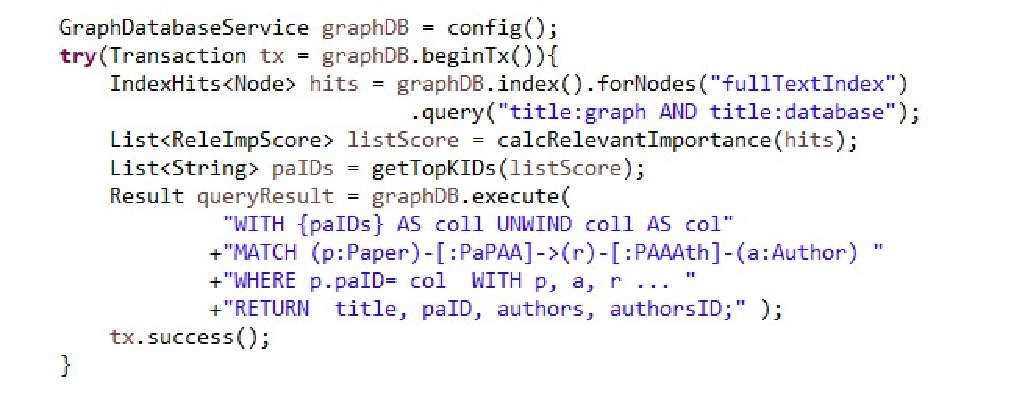
\includegraphics[width=\columnwidth]{queryProcess.pdf}
\vspace{-4.5ex}
\caption{Example workflow of \oursystem query engine}
\label{fig:queryProcess}
\vspace{-2ex}
\end{figure}




% visualization do what ?
% restful API
% scenarios, Query and Ranking Scholarly Entity, Author Profiling.
%Based on the graph storage, scholarly data was managed and processed in the system back-end. \oursystem collects user querys, dispatch to query engine and the results are then presented by visualizer using RESTful API. We employ Echarts (http://echarts.baidu.com/) to display scholarly article analysis and author profiling, detailed demonstrations are accessed in next section.
% function implement in back-end, echarts js  using RESTful API. demonstrate xxx in the next section.


%With scholarly data management and processing in the system back-end, the visualizer of \oursystem collects user queries through user interfaces. The queries are to the query engine and the returned results are then presented by visualizer. We will demonstrate some scholarly analysis scenarios in the next Section.


%\begin{table}[t!]
%%\begin{center}
%\caption{An example workflow of the query engine}
%\vspace{-1ex}
%\label{tab-workflow}
%\begin{scriptsize}
%\begin{tabular}{ l}
%%\hline
%%{An example workflow of the query engine} \\
%\hline
%1. GraphDatabaseService graphDB = new GraphDatabaseFactory()... ; \\
%2.  \hspace{0ex}  try(Transaction tx = graphDB.beginTx()) \{ \\
%3.  \hspace{4ex} 	IndexHits $\langle$ Node$\rangle$ hits = db.index().forNodes(``fullTextIndex") \\
%4.  \hspace{8ex}   .query("title: graph AND title:database"); \\
%5.  \hspace{4ex} 	List$\langle$ ReleImpScore$\rangle$ listScore = calcReleImpo(hits, ``graph database"); \\
%6.  \hspace{4ex} 	List$\langle$ String$\rangle$  paIDs = getTopKIDs(listScore); \\
%7.  \hspace{4ex}    Result result = graphDB.execute(`` \\
%8.  \hspace{8ex}		WITH \{paIDs\} AS IDs UNWIND IDs AS perID \\
%9.  \hspace{8ex}		MATCH (p:Paper)-[:PaToPAA]-$>$(r)-[:PAAToAut]-(a:Author)\\
%10.	\hspace{7ex}		WHERE p.paID= perID \\
%11. \hspace{7ex}        WITH p.title,  COLLECT(a.auName), SIZE(()-[:PaRef]-$>$(p)) AS cite, r \\
%12.	\hspace{7ex}		RETURN  paID, title, authors, cite ... ");\\
%13.	\hspace{4ex}	    tx.success();\\
%14. \hspace{2ex}  \} \\
%\hline
%\end{tabular} \\ %\vspace{.5ex}
%\end{scriptsize}
%%\end{center}
%\end{table}

